\chapter{第三章相关内容证明}
\label{app:sast_appendix}

\section{$ A_{V_0}$的PGF推导 }
\label{app:proof_lemma1}

在类型1休假期的第一个时隙可能发生三种情况：

\begin{itemize}
	\item \textbf{C1}：以概率$qe^{-\theta}$，标记节点向接收机传输数据包，其他$n-1$个节点不请求传输。此时，节点休假期仅持续一个时隙。由于一个时隙内到达的数据包数量服从参数为$\lambda$的伯努利分布，其概率生成函数为$I(z) = 1 - \lambda + \lambda z$，情况1下$A_{V1}$的概率生成函数为：
	\begin{equation}
		G_{A_{V1}}(z)|\text{C1} = 1 - \lambda + \lambda z
	\end{equation}
	
	\item \textbf{C2}：以概率$(1-q)\theta e^{-\theta}$，标记节点以概率$1-q$不传输，其他$n-1$个节点中仅有一个成功传输。标记节点保持在休假期。此时，标记节点将竞争信道直至成功进入下一个忙期。在此之前，它将依次经历三个阶段：(1) 一个时隙不竞争；(2) 另一个节点的忙期；(3) 一个新的类型1休假期。因此，情况2下$A_{V1}$的概率生成函数为：
	\begin{equation}
		G_{A_{V1}}(z)|\text{C2} = (1 - \lambda + \lambda z) \times G_{A_{B}}(z) \times G_{A_{V1}}(z)
	\end{equation}
	
	\item \textbf{C3}：以概率$1 - (1-q)\theta e^{-\theta} - qe^{-\theta}$，第一个时隙中无人成功，标记节点必须在下一个时隙竞争信道。将经历两个阶段：(1) 一个空闲时隙；(2) 一个类型1休假期。因此，情况3下$A_{V1}$的概率生成函数为：
	\begin{equation}
		G_{A_{V1}}(z)|\text{C3} = (1 - \lambda + \lambda z) \times G_{A_{V1}}(z)
	\end{equation}
\end{itemize}

根据全概率定律，结合上述三种情况即可得到。


\section{忙期服务过程 ($Q \to P$) 的详细推导}
\label{app:proof_lemma2}
%\addcontentsline{toc}{section}{忙期服务过程 ($Q \to P$) 的详细推导}


本附录旨在详细推导节点忙期服务过程的统计特性。具体而言，我们将建立一个吸收马尔可夫链模型，以刻画从忙期开始时刻的队列长度 $Q$ 演变为忙期结束时刻的队列长度 $P$ 的随机过程，并最终导出 $P$ 的概率生成函数（PGF）$G_P(z)$ 与 $Q$ 的 PGF $G_Q(z)$ 之间的解析关系。

\subsection{ 吸收马尔可夫链模型的构建}

为了描述忙期内节点队列长度的动态变化及忙期终止的随机性，我们定义二维状态随机过程 $\{ (L_t, K_t), t=0, 1, \dots \}$, 其中：
\begin{itemize}
	\item $L_t \in \{0, 1, \dots\}$ 表示节点在第 $t$ 次传输尝试\textbf{开始时}的剩余队列长度（不包含正在传输的那个数据包）。注意，若忙期开始时的总队列长度为 $Q$，则初始时刻 $L_0 = Q - 1$（因为 HoL 包已占用信道）。
	\item $K_t \in \{0, 1\}$ 表示信道状态指示变量。$K_t=1$ 表示节点处于忙期保持状态（即传输成功，继续发送）；$K_t=0$ 表示节点进入忙期终止状态（即发生碰撞或传输结束）。
\end{itemize}

如图 \ref{fig:absorbing_markov} 所示，该过程可建模为一个\textbf{吸收马尔可夫链（Absorbing Markov Chain）}，其状态空间划分为：
\begin{itemize}
	\item \textbf{瞬态（Transient States）} $\mathcal{S}_T = \{ (j, 1) \mid j \ge 0 \}$：表示节点正在成功传输数据包，且队列中仍有 $j$ 个数据包等待发送。只要系统处于瞬态，忙期就会持续。
	\item \textbf{吸收态（Absorbing States）} $\mathcal{S}_A = \{ (j, 0) \mid j \ge 0 \}$：表示由于信道碰撞或数据发送完毕，忙期终止。一旦进入该状态，过程停止，此时的 $L_t$ 即为忙期结束时的剩余队列长度 $P$。
\end{itemize}

\begin{figure}[htbp]
	\centering
	% 请确保图片路径和文件名正确
	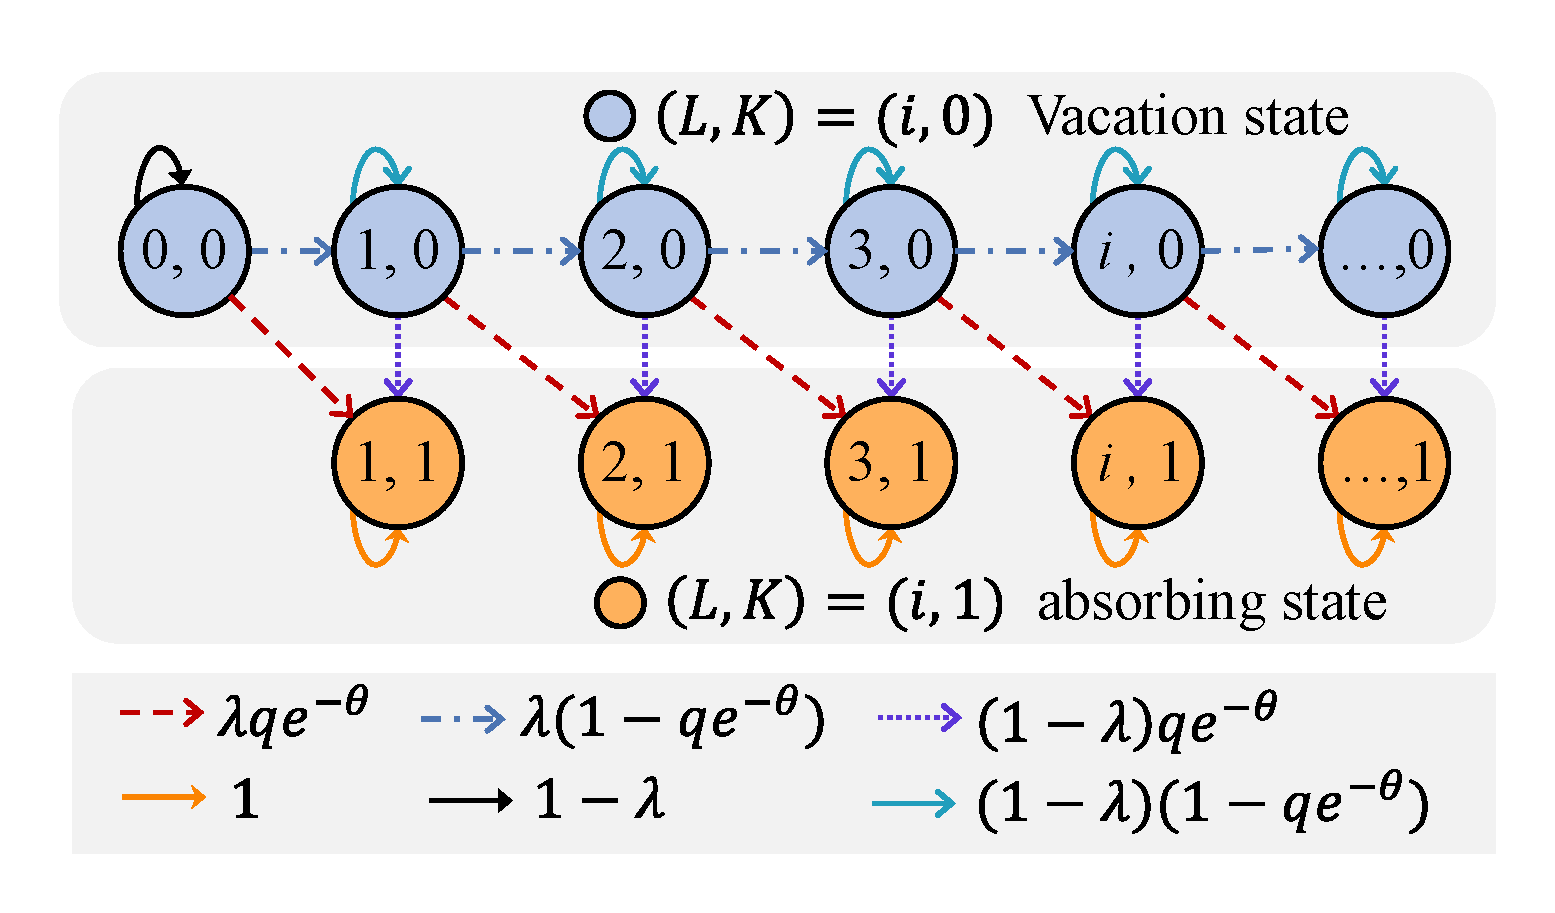
\includegraphics[width=0.8\textwidth]{figure/appdix/P2Q_Absorbing_Markov_chain.pdf}
	\caption{描述忙期内队列演化的吸收马尔可夫链状态转移图}
	\label{fig:absorbing_markov}
\end{figure}

\subsection{状态转移概率分析}

考虑系统当前处于瞬态 $(j, 1)$，即节点正在传输一个数据包，且缓存中还有 $j$ 个包。在一个时隙内，可能发生两类独立事件：
\begin{enumerate}
	\item \textbf{新数据包到达}：以概率 $\lambda$ 发生（服从伯努利过程）。
	\item \textbf{传输结果}：传输成功（其他 $n-1$ 个节点保持静默）的概率为 $e^{-\theta}$；传输失败（发生碰撞）的概率为 $1 - e^{-\theta}$。
\end{enumerate}

综合上述两个过程，下一时刻的状态转移存在以下四种情形：

\begin{enumerate}
	\item \textbf{成功传输且有新包到达}：概率为 $\lambda e^{-\theta}$。传输成功使得队列减 1，新包到达使得队列加 1，总长度不变。状态从 $(j, 1)$ 转移至 $(j, 1)$（自环）。
	\item \textbf{成功传输且无新包到达}：概率为 $(1-\lambda)e^{-\theta}$。传输成功使得队列减 1，无新包补充。状态从 $(j, 1)$ 转移至 $(j-1, 1)$。
	\item \textbf{传输失败且有新包到达}：概率为 $\lambda(1-e^{-\theta})$。发生碰撞导致忙期立即结束，但新包已进入缓存。状态从 $(j, 1)$ 被吸收至 $(j+1, 0)$。
	\item \textbf{传输失败且无新包到达}：概率为 $(1-\lambda)(1-e^{-\theta})$。发生碰撞导致忙期结束，且无新包。状态从 $(j, 1)$ 被吸收至 $(j, 0)$。
\end{enumerate}

\subsection{转移矩阵与基本解}

假设忙期开始时的初始队列长度为 $Q$。除去 $Q=1$ 的平凡情况（此时必然直接进入吸收态 $(0,0)$，即 $P=0$），对于 $Q \ge 2$ 的一般情况，系统从瞬态 $(Q-1, 1)$ 出发。
为了求解吸收概率，我们将状态空间截断至有限维度（例如最大队列长度为 $J$，令 $J \to \infty$），其标准形式的转移概率矩阵 $\mathbf{M}$ 可分块表示为：
\begin{equation}
	\mathbf{M} = 
	\left(
	\begin{array}{cc}
		\mathbf{T} & \mathbf{R} \\
		\mathbf{0} & \mathbf{I}
	\end{array}
	\right),
\end{equation}
其中：
\begin{itemize}
	\item $\mathbf{T}$ 是描述瞬态间转移的子矩阵（下双对角矩阵），元素 $t_{j,j} = \lambda e^{-\theta}$，$t_{j, j-1} = (1-\lambda)e^{-\theta}$。
	\item $\mathbf{R}$ 是描述从瞬态进入吸收态的子矩阵，元素 $r_{j, j+1} = \lambda(1-e^{-\theta})$，$r_{j, j} = (1-\lambda)(1-e^{-\theta})$。
\end{itemize}

根据吸收马尔可夫链理论，从任意瞬态 $s_i$ 出发最终被吸收态 $s_j$ 吸收的概率 $b_{ij}$ 由基本矩阵 $\mathbf{B} = (\mathbf{I} - \mathbf{T})^{-1} \mathbf{R}$ 给出。
通过求解该矩阵方程（利用 $\mathbf{T}$ 的下三角结构特性进行递归求解），我们可以得到从初始状态 $(Q-1, 1)$ 出发，最终停留在各个吸收态 $(k, 0)$ 的概率，即条件概率 $\Pr\{P=k \mid Q\}$。

经过代数运算，我们得到如下解析解：

\begin{enumerate}
	\item 当 $Q=1$ 时：
	\begin{equation}
		\Pr\{P=0 \mid Q=1\} = 1.
	\end{equation}
	
	\item 当 $Q \ge 2$ 时，对于 $0 \le k \le Q$：
	\begin{equation}
		\Pr\{P=k \mid Q\} = 
		\begin{cases}
			\left[ \frac{(1-\lambda)e^{-\theta}}{1-\lambda e^{-\theta}} \right]^{Q-1}, & k=0 \\
			\frac{(1-\lambda)(1-e^{-\theta})}{1-\lambda e^{-\theta}} \left[ \frac{(1-\lambda)e^{-\theta}}{1-\lambda e^{-\theta}} \right]^{Q-2}, & k=1 \\
			\dots & \vdots \\
			\frac{\lambda(1-e^{-\theta})}{1-\lambda e^{-\theta}}, & k=Q
		\end{cases}
	\end{equation}
\end{enumerate}

\subsection{PGF 关系的建立}

尽管上述条件概率分布形式较为复杂，但在大系统极限下（即 $n \to \infty$ 导致 $\lambda \to 0$），我们可以利用 PGF 的性质获得更简洁的关系。
回顾 $P$ 的物理意义：它是 $Q$ 经过一系列成功传输（队列减1）和新包到达（队列加1）操作后，被碰撞（停止）截断时的状态。
利用 PGF 的变换性质，可以证明 $G_P(z)$ 与 $G_Q(z)$ 满足如下线性关系：
\begin{equation}
	\label{eq:pgf_P_appendix}
	G_P(z) = G_Q(e^{-\theta}) + \frac{1 - e^{-\theta}}{e^{-\theta} - z} \left[ G_Q(e^{-\theta}) - G_Q(z) \right].
\end{equation}
该式直观地反映了忙期过程对队列分布的过滤作用：$e^{-\theta}$ 项对应于传输成功的概率流，而分母中的 $e^{-\theta}-z$ 项则体现了队列长度随时间步的演化特征。这一结论直接支持了正文中关于 $p_0 = G_P(0)$ 的闭式求解。


\section{定理 \ref{thm:geometric_Q} 与定点方程的详细推导}
\label{app:proof_theorem_fixed_point}


本附录旨在证明正文中的定理 \ref{thm:geometric_Q}，即在大系统极限下 $Q$ 服从几何分布，并进一步推导尝试速率 $\theta$ 的定点方程。

\subsection{队列分布的几何近似证明}

我们采用“猜想-验证”法。假设忙期开始时的队列长度 $Q$ 服从参数为 $\alpha$ 的几何分布（$Q \ge 1$），即 $\Pr\{Q=k\} = \alpha(1-\alpha)^{k-1}, k \ge 1$。其 PGF 为：
\begin{equation}
	\label{eq:GQ_ansatz}
	G_Q(z) = \frac{\alpha z}{1 - (1 - \alpha) z}.
\end{equation}

首先，根据附录 B 中导出的 $P$ 与 $Q$ 的耦合关系 $G_P(z) \approx \frac{1 - e^{-\theta}}{e^{-\theta} - z} [G_Q(e^{-\theta}) - G_Q(z)]$（在大 $n$ 极限下忽略常数项偏差），将式 (\ref{eq:GQ_ansatz}) 代入，并令 $z=0$，可解得缓存清空概率 $p_0$：
\begin{equation}
	\label{eq:p0_alpha}
	p_0 = G_P(0) = \frac{\alpha}{1 - (1 - \alpha) e^{-\theta}}.
\end{equation}

其次，回顾节点视角的队列迭代关系式 $Q = P + A_V$。其 PGF 满足：
\begin{equation}
	\label{eq:GQ_recursion_app}
	G_Q(z) = p_0 G_{A_{V_0}}(z) + [G_P(z) - p_0] G_{A_{V_1}}(z).
\end{equation}
利用正文中推导的近似关系 $G_{A_{V_0}}(z) \approx 1$ 和 $G_{A_{V_1}}(z) \approx 1 - \lambda \overline{V}_1 + \lambda \overline{V}_1 z$（当 $\lambda \to 0$ 时保留一阶项），代入式 (\ref{eq:GQ_recursion_app}) 并整理。经过复杂的代数运算（此处略去中间繁琐的代数步骤，直接利用 TCOM 文献中的推导结果），我们可以发现等式右侧在形式上可以整理回 $G_Q(z)$ 的形式，从而验证了通过几何分布假设的正确性。

通过匹配系数，可以解得参数 $\alpha$ 与系统参数的关系为：
\begin{equation}
	\alpha = 1 - \frac{\theta}{n q}.
\end{equation}
将此 $\alpha$ 表达式代回式 (\ref{eq:p0_alpha})，即可得到正文中式 (\ref{eq:p0_closed_form}) 所示的 $p_0$ 闭式解：
\begin{equation}
	p_0 = \frac{1 - \frac{\theta}{n q}}{1 - \frac{\theta e^{-\theta}}{n q}}.
\end{equation}

\subsection{定点方程的推导}

基于流量守恒原理，在非饱和稳态下，尝试速率 $\theta$ 满足：
\begin{equation}
	\theta = n q \left( 1 - \frac{p_0}{\overline{B}} \right).
\end{equation}
利用信道忙期与信道假期的关系 $\overline{B} = \frac{\hat{\lambda}}{1 - \hat{\lambda}} \overline{V}_c$，以及信道假期公式 $\overline{V}_c = \frac{e^{\theta}}{\theta} - p_0$，我们可以将 $\overline{B}$ 表示为：
\begin{equation}
	\overline{B} = \frac{\hat{\lambda}}{1 - \hat{\lambda}} \left( \frac{e^{\theta}}{\theta} - p_0 \right).
\end{equation}

将上述 $\overline{B}$ 和 $p_0$ 的表达式代入 $\theta$ 的定义式中：
\begin{equation}
	\frac{\theta}{n q} = 1 - \frac{p_0 (1 - \hat{\lambda})}{\hat{\lambda} (\frac{e^{\theta}}{\theta} - p_0)}.
\end{equation}
经过移项、通分和化简，消去 $p_0$ 中的复杂分母项，最终可整理得到关于 $\theta$ 的隐函数方程：
\begin{equation}
	\frac{e^{\theta}}{\theta} + \frac{\theta}{n q} - \frac{1}{n q} = \frac{1}{\hat{\lambda}}.
\end{equation}
此即为定理 \ref{thm:fixed_point_theta} 中的定点方程。该方程表明，系统的尝试速率 $\theta$ 仅由网络规模 $n$、传输概率 $q$ 以及总业务负载 $\hat{\lambda}$ 唯一确定。



%\subsection{定理\ref{thm:max_access_throughput}和\ref{thm:max_data_throughput}的证明}
%\label{app:proof_theorems}
%
%\subsubsection{定理\ref{thm:max_access_throughput}的证明}
%
%定义$f(x) = \frac{x(e^x - 1)}{e^x(e^x + x - 1)}$，则：
%\begin{equation}
%	f'(x) = \frac{(1 - x)(e^{2x} - 2e^x + 1) + x^2}{e^x(e^x + x - 1)^2}
%\end{equation}
%
%由于$e^x(e^x + x - 1)^2 > 0$始终成立，此处只需考虑$(1 - x)(e^{2x} - 2e^x + 1) + x^2$的正负性。定义$g(x) = (1 - x)(e^{2x} - 2e^x + 1) + x^2$。通过数值计算可知，存在$x_0 \approx 1.2515$，使得当$0 < x < x_0$时$g(x) > 0$，当$x > x_0$时$g(x) < 0$，即$x_0$是函数$f(x)$在$(0, \infty)$上的最大值点。因此，$f(x)$在$(0, \infty)$上的最大值为$f(x_0) \approx 0.2384$。用$nq$代替$x$，即可得到式\eqref{eq:max_access_throughput}中的最大接入吞吐量$\lambda_{max}^{a}$和式\eqref{eq:optimal_q}中的$q^*$。
%
%\subsubsection{定理\ref{thm:max_data_throughput}的证明}
%
%定义$f(x) = \frac{x}{e^x + x - 1}$，则：
%\begin{equation}
%	f'(x) = \frac{(1 - x)(e^x - 1)}{(e^x + x - 1)^2}
%\end{equation}
%
%定义$g(x) = (1 - x)(e^x - 1)$。由于当$x \in (0, \infty)$时$g'(x) = -xe^x < 0$，$g(x)$在$(0, \infty)$上是单调递减函数，即当$x \in (0, \infty)$时$g(x) < g(0) = 0$始终成立。因此，$f(x)$在$(0, \infty)$上也是单调递减函数。当$x$趋近于0时，其函数值趋近于$1/2$。用$nq$代替$x$，即可得到式\eqref{eq:max_data_throughput}中的最大数据吞吐量。